\chapter{Das Programm}\label{the_program}

In diesem Kapitel werden wir auf die Implementierung von Netzwerk \ref{net_sltr} aus dem vorherigen Abschnitt eingehen. Das im Folgenden beschriebene Programm baut auf Vermutung \ref{int_conj} -- dass sich aus jedem nicht ganzzahligen zulässigen Fluss auf Netzwerk \ref{net_sltr} ein Gutes-FAA extrahieren lässt -- auf. Der Code wurde in SageMath geschrieben und ist auf Anfrage erhältlich \cite{sage}. Algorithmus \ref{algo_gfaa} gibt einen Überblick der durchgeführten Schritte bei der Suche nach einem Guten-FAA für einen gegebenen ebenen intern-3-zusammenhängenden Graphen mit Aufhängungen $\{a_1,a_2,a_3\}$.


\begin{algorithm}
	\SetKwInOut{Input}{Input}
	\SetKwInOut{Output}{Output}
	\underline{Good-FAA} $(G,f_{aus},sus)$\;
	\Input{$G$, a planar, internally-3-connected Graph, $f_{aus}$, the outer face and $sus = \{a_1,a_2,a_3\}$ the suspensions.}
	\Output{A Good-FAA for G if possible}
	\If{$G_{sus}$ has FAA}
		{
        		Initialize $\mathcal{N}_G$ \;
        		$(d_1,d_2) \longleftarrow$ Demands for $\mathcal{N}_G$ \;
        		$\varphi = (\varphi_1,\varphi_2) \longleftarrow$ Multicomodity-Flow($\mathcal{N}_G$) \;
        		\If{$|\varphi_1| = d_1$ and $|\varphi_2| = d_2$}
        			{
        			$\phi \longleftarrow$ Good-FAA from $\varphi_2$ \;
			return: $\phi$
			}
		}
		\caption{An algorithm to detect and return a Good-FAA for a plane, internally-3-connected and suspended Graph $G$.}
\end{algorithm}


Die Kontrolle, ob für $G$ ein FAA existiert, ist optional, lässt sich jedoch, zum Beispiel wie zuvor über ein 1-Fluss-Problem, in polynomineller Zeit auf einem deutlich kleineren Netzwerk bestimmen. Dies spart Zeit, falls zu Aufhängungen keine FAAs auf $G$ existieren. Das Multi-Fluss-Problem auf $\mathcal{N}_G$ zu gegebenen Bedarfen $(d_1,d_2)$ wird mithilfe des in SageMath enthaltenen Solvers \textit{Glpk} für Lineare Programmierung gelöst, welcher ein Paar von Flussgraphen $(\varphi_1,\varphi_2)$ ausgibt, falls eine zulässige Lösung existiert und sonst nichts\cite{glpk,sage}. In den Zeilen \ref{int_one_flow1} und \ref{int_two_flow1} wird, im Gegensatz zu Zeile \ref{two_flow1}, nur nach ganzzahligen Lösungen gesucht. Aus einer ganzzahligen Lösung kann man ein FAA $\phi$ aus $\varphi_2$ extrahieren, indem man die Zuweisungs-Pfade durch die Dummy-Senke zurück verfolgt. Wir betreten jeden passierten Dummy-Knoten $v^*$ aus einem Winkel $(f,v)$. Diese Winkel ergeben die Zuweisungen $\phi$.

Die Überprüfung ab Zeile \ref{algo_check} ist unter der Annahme, dass Vermutung \ref{int_conj} stimmt, nicht notwendig. Es könnte hier ein FAA aus $\varphi_2$ extrahiert und ausgegeben werden. Wir gewährleisten jedoch so die Korrektheit des Algorithmus, weil wir den Beweis von Vermutung \ref{int_conj} noch nicht gefunden haben. Bei Tests ergaben sich mit diesem Ansatz immer noch deutlich kürzere Berechnungszeiten als bei der Suche nach ausschließlich ganzzahligen Lösungen. Zeile \ref{sanity_check} sollte nach Vermutung \ref{faa_conj} nicht erreicht werden. Sie stellt jedoch sicher, dass Algorithmus \ref{algo_gfaa} immer dann ein Gutes-FAA ausgibt, wenn ein ganzzahliger Fluss auf Netzwerk \ref{net_sltr} existiert.

\begin{remark}
In der Implementierung wurden die Kanten innerhalb von Gebieten $f$ mit $|f|=3$ weggelassen, da die einzig mögliche Lösung hier ist, dass nur drei Ecken-Pfade durch das Gebiet laufen. Die Bedarfe werden dementsprechend angepasst.
\end{remark}

\section{Visualisierung}

Nehmen wir an, wir haben für einen Graphen $G$ ein Gutes-FAA $\phi$ gefunden. Für eine SLTR müssen wir eine zu $\phi$ passende Einbettung von $G$ finden. Wir werden den in Abschnitt \ref{harmonic_approach} erörterten Ansatz über harmonische Funktionen nutzen, um eine SLTR von $G$ zu erhalten.

Wir wollen nun eine Einbettung $f:V\to \mathbb{R}^2$ von $G$ ähnlich der Gummiband-Repräsentation berechnen, die $\phi$ respektiert. Sei $S \subseteq V$ die Menge der Knoten von $f_{aus}$. Nach Abschnitt \ref{harmonic_approach} gelten die folgenden harmonischen Gleichungen für zugewiesene (oben) und nicht zugewiesene Knoten (unten).

$$ f(v) = \lambda_v f(u) + (1-\lambda_v)f(w) \text{, mit } \lambda_v \in (0,1) $$
$$ f(v) = \sum_{u \in N(v)} \lambda_{uv} f(u) \text{, mit }  \sum_{u \in N(v)}\lambda_{uv} = 1 \text{ und } \lambda_{uv} > 0 $$

Um zu einer gegebenen Gewichtsfunktion $\lambda$ eine Lösung zu finden, können wir diese Gleichungen um die Bilder der Aufhängungen $f(A) = f(\{a_1,a_2,a_3\})$ erweitern und als Matrix schreiben.

\[ M_{\lambda}(\vec{v_x},\vec{v_y}) = \big( \begin{smallmatrix}f(A)_x&f(A)_y\\ 0&0\end{smallmatrix} \big) \text{, mit } (M_{\lambda})_{vw} =
	\begin{dcases}
	-\lambda_{vw} & \text{falls } (v,w) \in E, \\
	\textstyle\sum_{u \in N(v)} \lambda_{uv} & \text{falls } v = w, \\
	0 & \text{sonst.} \\
	\end{dcases}
\]

Wenn wir nun die Pseudo-Inverse berechnen, erhalten wir eine Einbettung.

$$f(V) = M_{\lambda}^{-1}\big( \begin{smallmatrix}f(A)_x&f(A)_y\\ 0&0\end{smallmatrix} \big).$$

Wir wollen nun, inspiriert von den \textit{iterativen Tutte Einbettungen} nach Felsner und Scheucher, diese Rechnung mehrmals durchführen und Schritt für Schritt die Gewichtung $\lambda$ anpassen \cite{fs17}. Wünschenswert wäre es, wenn sich die Zeichnung nach einer gewissen Anzahl an Schritten nur noch so wenig verändert, dass wir den Algorithmus abbrechen können und die letzte Zeichnung ausgeben.

\subsection{Probleme bei der Wahl von $\lambda$}

Setzten wir im ersten Durchlauf $\lambda = 1$, erhalten wir eine klassische Gummiband-Repräsentation, die $\phi$ respektiert. Wir wollen nun anhand dieser Einbettung $\lambda$ verändern, um Iteration für Iteration, eine \glqq schönere\grqq{ } Einbettung zu erhalten. Halten wir zwei Punkte fest, die wir als Bewertungsmaßstab für eine schöne Einbettung berücksichtigen können.

\begin{itemize}
\item Es gibt keine zu großen oder zu kleinen Gebiete.
\item Es existieren keine zu kurzen Kanten.
\end{itemize}

Sehr lange Kanten lassen sich, wie in Beispiel \ref{bsp_large_corner}, nicht immer vermeiden. Es gibt SLTRs, wie in Beispiel \ref{bsp_long_segment}, bei denen alle inneren Knoten zugewiesen sind. Dies macht eine gute Wahl der $\lambda$ kompliziert. Der Ansatz nach Scheucher \cite{fs17}, bei dem $\lambda$ als monoton steigende Funktion proportional zu Größe der an eine Kante angrenzenden Gebiete und ihrer Länge gewählt wird, konvergiert im Allgemeinen nicht und liefert so auch keine schönen Zeichnungen. Allgemein wurden besonders SLTRs mit wenigen Kanten betrachtet, da für diese die oben erwähnten Einschränkungen stärker auftreten.

\begin{example}\label{bsp_long_segment}
Bei der in Abbildung \ref{long_segment} a) zu sehenden SLTR sind alle Knoten, bis auf die Aufhängungen, einem Gebiet zugeordnet. Somit liegt jeder Knoten auf einer Gerade und es existieren nur Gleichungen vom Typ

$$ f(v) = \lambda_v f(u) + (1-\lambda_v)f(w) \text{, mit } \lambda_v \in (0,1).$$

Um von der linken zur rechten Zeichnung zu gelangen, wollen wir das Gebiet unten in der Mitte verkleinern, doch die drei angrenzenden Kanten kommen in keiner der Gleichungen zu Bestimmung unserer Einbettung $f(V)$ vor. Die Kanten, die uns helfen können, das Segment in rot nach unten zu bewegen und somit das untere Dreieck zu verkleinern, sind in blau eingefärbt. Um zur Zeichnung auf der rechten Seite zu gelangen, erfolgt die Wahl der $\lambda$ in jedem Schritt nach folgenden Schema. Wir berechnen zu jedem Segment die Mengen der Kanten $S_1,S_2$, die an Gebieten liegen die vollständig auf einer der beiden Seiten des Segments liegen. Parallel dazu berechnen wir die Summe der Flächen dieser Gebiete $A_1,A_2$. Falls beide Mengen nicht leer sind, erhöhen wir für jede Kante $e \in S_i$ $\lambda(e)$ um $a_i$ mit:

$$ a_i = A_i^{1.25}*|A_j|^{-2} \text{ , mit } j \neq i.$$

Die Exponenten sind heuristisch gewählt. Wir brechen entweder ab, wenn die Einbettung konvergiert oder wir eine feste Anzahl an Schritten durchgeführt haben. Eine so errechnete Einbettungen ist in Abbildung \ref{long_segment} c) zu sehen.
\end{example}

\begin{figure}[h]
	\centering
  \includegraphics[width=1\textwidth]{example1_vis.pdf}
  \caption{a) Eine Einbettung mit $\lambda$=1. b) Eine Einbettung nach bei der wir nur zu $e$ adjazente Gebiete für $\lambda(e)$ berücksichtigen. c) Eine Einbettung nach dem Schema aus Beispiel \ref{bsp_large_corner}.}
  \label{long_segment}
\end{figure}

Dieser Ansatz führt aber, gerade bei Graphen mit vielen Knoten, zu keiner Zeichnung die die oben genannten Punkte erfüllt (vergleiche Abbildung \ref{large_corner}, b)). Wir betrachten ein weiteres Beispiel um ein zweites Schema zu erläutern.

\begin{example}\label{bsp_large_corner} 
Gerade für Graphen mit vielen Knoten führt der Ansatz aus Beispiel \ref{bsp_long_segment} nicht immer zu einer schönen Zeichnung der SLTR. In Abbildung \ref{large_corner} a) ist so ein Graph mit der ersten, für $\lambda=1$, erhaltenen Zeichnung und dem Resultat nach 50 Schritten nach dem Schema aus Beispiel \ref{bsp_long_segment} zu sehen (Abbildung \ref{large_corner} b). Ein anderer iterativer Ansatz führt hier jedoch zu schöneren Ergebnissen. Wir setzen bei der Initialisierung $\lambda_0(e)=2$ für jede Kante von $G$. Nun multiplizieren wir die Kanten an den Gebieten $f$ mit $A(f) > A(f_{max})*(1+\epsilon)$ mit einer Konstante $c \in \mathbb{N}$. Für diese Kanten gilt somit $\lambda_{i+1}(e) = \lambda_{i}(e)*c$. Wir wählen $\epsilon = 0,1$ und $c=2$. In Abbildung \ref{large_corner} c) ist die Einbettung nach 50 Schritten zu sehen.
\end{example}

\begin{figure}[h]
	\centering
  \includegraphics[width=1\textwidth]{example1_vis.pdf}
  \caption{Drei Zeichnungen der gleichen SLTR für unterschiedliche $\lambda$. a) Für $\lambda=1$. b) Nach dem Ansatz aus Beispiel \ref{bsp_long_segment}. c) Nach dem Ansatz aus Beispiel \ref{bsp_long_segment}.}
  \label{large_corner}
\end{figure}

\subsection{Eine heuristisch gute Wahl von $\lambda$}

Der Ansatz aus Beispiel \ref{bsp_large_corner} führt jedoch auch bei einigen Graphen zu unschönen Zeichnungen. Ein Kompromiss aus beiden, hat heuristisch vielversprechende Zeichnungen erzeugt. Wir führen die beiden Algorithmen hintereinander aus. Falls das Schema aus Beispiel \ref{bsp_long_segment} konvergiert, brechen wir ab und geben die Zeichnung aus. Falls nicht, speichern wir die berechneten Werte $\lambda'$ und führen das Schema aus Beispiel \ref{bsp_large_corner} durch. Bei jedem Schritt berechnen wir nun eine neue Zeichnung mit $\lambda(e) = \lambda_{i+1}(e) + \lambda'(e)$. Wieder führen wir 50 Schritte durch.  TODO

Beispiele von so errechneten Zeichnungen verschiedener SLTRs sind in Abbildung \ref{vis_examples} zu sehen.

\section{Experimentelle Rechnungen}\label{stats}

Es folgt eine kurze statistische Betrachtung der Verteilung von Graphen mit SLTRs. Hier würde eine gleichmäßige Wahl von (intern-)3-zusammenhängenden Graphen die aufschlussreichsten Resultate liefern. Ein Algorithmus zur zufälligen Erstellung 3-zusammenhängender planarer Graphen lässt sich zum Beispiel nach einem Ansatz von Fusy implementieren \cite{fusy09}. Als Teilschritt der Erstellung eines uniformen Samplers für planare Graphen werden hier 3-zusammenhängende planare Graphen mit gleichverteilter Wahrscheinlichkeit erzeugt. Die Implementierung ist jedoch aufgrund der notwendigen Auswertung von Erzeugendenfunktionen kompliziert. Diese Analyse beschränkt sich daher auf pseudo-zufällig erzeugte Graphen. 

Es folgt eine kurze Beschreibung des von uns benutzen Samplers. Wir beginnen mit einem $K_4$. Nun wird in jedem Schritt mit noch zu wählenden Wahrscheinlichkeiten eine der folgenden vier Operationen durchgeführt.

\begin{itemize}
\item[PG1] Ein Knoten $v$ mit deg$(v) \geq 4$ wird in $v_1,v_2$ geteilt und eine Kante $(v_1,v_2)$ eingefügt. Nun werden die zyklisch sortierten Nachbarn in zwei Teile $N_1,N_2$ getrennt und mit $v_1$ beziehungsweise $v_2$ verbunden.
\item[PG2] Eine Knoten wird auf einer Kante eingefügt und mit einem in einem angrenzenden Gebiet liegenden Knoten verbunden.
\item[PG3] Ein Knoten wird in ein Gebiet eingefügt und mit mindestens drei der am Gebiet liegenden Knoten verbunden. 
\item[PG4] Es wird eine zufällige Kante in ein Gebiet mit mehr als drei Knoten eingefügt.
\end{itemize}


safasdasd
\begin{figure}
        \centering
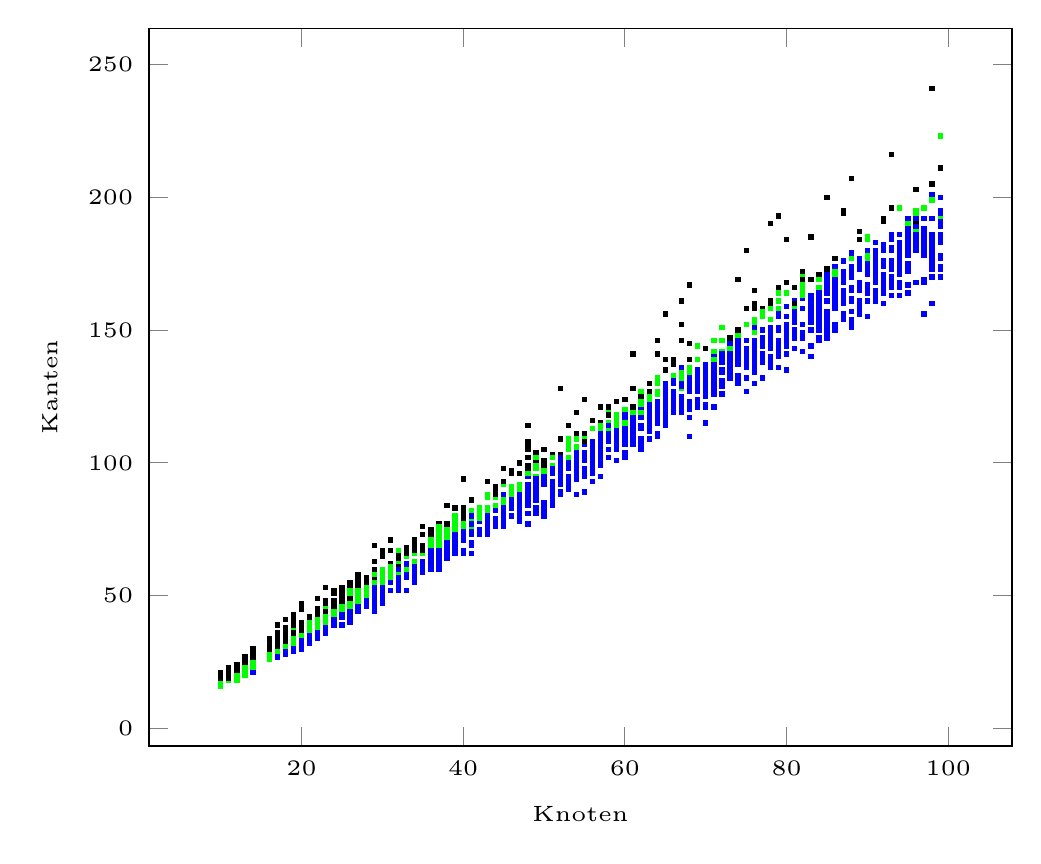
\begin{tikzpicture}[thick, scale=1.6,font=\tiny]
\begin{axis}[xlabel=Knoten,ylabel=Kanten]

\addplot[
	scatter/classes={
    	s={mark=square*,scale=0.2,black},
    	f={mark=square*,scale=0.2,green},
    	n={mark=square*,scale=0.2,blue}
    	},
	scatter,only marks,
    	scatter src=explicit symbolic,]
	table[meta=label] {
x y label
10 18 s
10 16 f
10 19 s
10 19 s
10 19 s
10 20 s
10 18 s
10 18 s
10 17 s
10 19 s
10 19 s
10 21 s
10 17 f
10 17 s
10 18 s
10 20 s
10 16 f
10 20 s
10 17 f
10 16 f
11 19 s
11 22 s
11 19 s
11 19 f
11 19 s
11 22 s
11 18 f
11 20 s
11 22 s
11 19 s
11 20 s
11 21 s
11 19 s
11 20 s
11 20 f
11 18 f
11 20 s
11 23 s
11 20 s
11 19 s
12 18 f
12 22 s
12 22 s
12 18 f
12 20 f
12 23 s
12 21 s
12 22 s
12 19 f
12 24 s
12 22 s
12 20 f
12 20 f
12 21 s
12 18 f
12 22 s
12 21 s
12 24 s
12 20 f
12 18 f
13 21 f
13 20 f
13 20 f
13 25 s
13 22 f
13 26 s
13 20 f
13 27 s
13 25 s
13 24 s
13 24 s
13 24 s
13 25 s
13 27 s
13 23 s
13 24 s
13 26 s
13 25 s
13 23 f
13 26 s
14 29 s
14 30 s
14 21 n
14 23 f
14 24 f
14 23 f
14 27 s
14 27 s
14 27 s
14 30 s
14 28 s
14 27 s
14 25 s
14 25 s
14 28 s
14 25 s
14 29 s
14 25 s
14 25 s
14 25 f
16 29 f
16 26 f
16 27 f
16 28 f
16 31 s
16 30 s
16 31 s
16 31 s
16 32 s
16 33 s
17 31 s
17 31 f
17 33 s
17 28 f
17 31 f
17 32 s
17 32 s
17 32 s
17 30 f
17 33 s
18 34 s
18 37 s
18 33 s
18 33 s
18 29 n
18 30 f
18 30 f
18 37 s
18 36 s
18 34 s
19 36 s
19 30 n
19 30 n
19 39 s
19 38 s
19 34 f
19 33 f
19 39 s
19 30 n
19 43 s
20 30 n
20 32 n
20 40 f
20 37 f
20 38 f
20 34 f
20 45 s
20 31 n
20 37 s
20 38 s
21 42 s
21 40 f
21 42 s
21 37 f
21 33 n
21 32 n
21 37 f
21 37 f
21 35 n
21 42 s
22 34 n
22 39 f
22 40 f
22 41 s
22 45 s
22 49 s
22 36 n
22 42 s
22 41 f
22 42 s
23 46 s
23 38 n
23 44 f
23 42 f
23 46 s
23 45 s
23 45 s
23 42 f
23 48 s
23 47 s
24 45 s
24 40 n
24 42 n
24 45 f
24 45 f
24 52 s
24 42 f
24 47 f
24 48 s
24 44 f
25 43 n
25 53 s
25 47 s
25 50 s
25 49 s
25 43 n
25 43 n
25 49 s
25 44 n
25 46 f
26 47 f
26 49 f
26 48 f
26 49 f
26 49 f
26 52 f
26 48 f
26 44 n
26 51 f
26 46 n
27 53 f
27 50 f
27 55 f
27 48 f
27 45 n
27 57 s
27 52 s
27 56 s
27 46 n
27 54 s
28 48 n
28 54 s
28 51 f
28 52 f
28 52 f
28 48 n
28 46 n
28 56 s
28 55 s
28 49 n
29 50 n
29 69 s
29 54 f
29 56 s
29 58 s
29 57 s
29 63 s
29 44 n
29 53 f
29 55 f
16 33 s
16 27 f
16 30 f
16 28 f
16 29 f
16 29 s
16 31 s
16 28 f
16 34 s
16 30 s
16 28 f
16 32 s
16 27 f
16 30 s
16 26 f
16 28 f
16 30 s
16 30 s
16 28 f
16 28 f
17 31 f
17 30 f
17 39 s
17 32 s
17 33 s
17 35 s
17 31 s
17 27 n
17 35 s
17 27 n
17 31 f
17 29 f
17 33 s
17 34 s
17 30 f
17 39 s
17 31 s
17 29 f
17 36 s
17 33 s
18 29 n
18 36 s
18 38 s
18 30 f
18 41 s
18 34 s
18 31 f
18 33 f
18 31 f
18 36 s
18 33 f
18 29 n
18 30 f
18 29 n
18 33 s
18 28 n
18 37 s
18 34 s
18 37 s
18 37 s
19 33 f
19 32 f
19 37 s
19 35 f
19 33 f
19 31 n
19 31 n
19 35 f
19 38 s
19 34 f
19 41 s
19 37 f
19 33 f
19 29 n
19 35 f
19 40 s
19 36 s
19 30 n
19 32 f
19 34 f
20 36 f
20 39 f
20 40 s
20 47 s
20 37 f
20 36 f
20 33 n
20 36 f
20 38 s
20 36 f
20 40 s
20 30 n
20 36 f
20 37 f
20 33 n
20 37 s
20 33 n
20 32 n
20 40 s
20 38 s
21 40 f
21 40 s
21 34 n
21 37 f
21 40 s
21 40 s
21 37 f
21 34 n
21 39 f
21 39 f
21 38 f
21 42 s
21 40 f
21 38 f
21 37 f
21 39 f
21 40 s
21 34 n
21 40 f
21 42 s
22 38 f
22 37 n
22 38 n
22 45 s
22 39 f
22 40 f
22 34 n
22 42 f
22 37 n
22 41 f
22 41 f
22 35 n
22 38 f
22 43 s
22 40 f
22 34 n
22 40 f
22 36 n
22 43 s
22 36 n
23 36 n
23 47 s
23 42 f
23 36 n
23 36 n
23 46 s
23 42 f
23 43 s
23 42 f
23 38 n
23 53 s
23 45 f
23 48 s
23 48 s
23 45 f
23 43 f
23 44 s
23 47 s
23 40 f
23 40 f
24 42 n
24 47 s
24 44 f
24 43 f
24 47 s
24 41 n
24 43 f
24 51 s
24 39 n
24 46 f
24 40 n
24 47 s
24 51 s
24 41 n
24 46 f
24 45 f
24 41 n
24 44 f
24 46 s
24 46 s
25 42 n
25 43 n
25 51 s
25 52 s
25 50 s
25 47 f
25 47 f
25 44 f
25 49 s
25 48 f
25 45 f
25 44 f
25 39 n
25 45 f
25 50 s
25 48 s
25 45 f
25 50 s
25 51 s
25 43 n
26 42 n
26 47 n
26 55 s
26 47 f
26 46 f
26 43 n
26 50 s
26 42 n
26 50 f
26 48 f
26 44 n
26 40 n
26 54 s
26 45 n
26 49 s
26 45 n
26 46 f
26 47 f
26 47 f
26 46 f
27 52 s
27 48 f
27 54 s
27 58 s
27 44 n
27 51 f
27 51 f
27 52 s
27 47 n
27 52 f
27 45 n
27 48 f
27 45 n
27 51 f
27 46 n
27 52 f
27 44 n
27 51 f
27 51 f
27 48 f
28 47 n
28 50 f
28 57 s
28 48 n
28 48 n
28 56 s
28 47 n
28 51 n
28 46 n
28 55 s
28 46 n
28 55 s
28 48 n
28 48 n
28 54 s
28 51 n
28 52 f
28 53 f
28 50 f
28 56 s
29 56 s
29 56 s
29 52 n
29 53 n
29 59 s
29 51 n
29 46 n
29 55 f
29 51 n
29 63 s
29 63 s
29 60 s
29 48 n
29 48 n
29 46 n
29 47 n
29 51 n
29 58 f
29 60 s
29 49 n
30 67 s
30 65 s
30 53 n
30 59 s
30 47 n
30 53 n
30 56 f
30 51 n
30 49 n
30 59 s
30 54 f
30 55 f
30 59 s
30 59 f
30 49 n
30 57 f
30 53 n
30 60 f
30 56 f
30 56 f
31 61 s
31 62 f
31 62 s
31 60 s
31 52 n
31 67 s
31 55 n
31 59 f
31 57 f
31 56 f
31 56 n
31 57 f
31 58 f
31 71 s
31 52 n
31 61 s
31 55 n
31 61 f
31 58 f
31 55 n
32 67 f
32 59 n
32 61 f
32 54 n
32 55 n
32 62 s
32 59 f
32 57 n
32 62 s
32 60 f
32 56 n
32 65 s
32 57 n
32 63 f
32 52 n
32 64 s
32 56 n
32 59 f
32 60 n
32 64 s
33 58 n
33 62 f
33 59 n
33 58 n
33 59 n
33 68 s
33 66 s
33 62 f
33 60 f
33 67 s
33 52 n
33 62 f
33 57 n
33 62 n
33 58 n
33 58 n
33 65 f
33 66 s
33 60 f
33 68 s
34 63 f
34 67 s
34 71 f
34 58 n
34 70 f
34 60 n
34 61 n
34 55 n
34 70 s
34 63 f
34 67 f
34 63 f
34 68 s
34 59 n
34 66 f
34 56 n
34 67 s
34 59 n
34 71 s
34 69 s
35 73 s
35 66 n
35 59 n
35 67 f
35 66 f
35 69 f
35 68 s
35 61 n
35 61 n
35 76 s
35 69 s
35 67 f
35 59 n
35 63 n
35 68 s
35 59 n
35 67 s
35 69 s
35 59 n
35 63 n
36 62 n
36 65 n
36 62 n
36 65 n
36 62 n
36 60 n
36 61 n
36 70 f
36 64 n
36 73 s
36 71 f
36 65 n
36 65 n
36 62 n
36 65 n
36 68 f
36 75 s
36 63 n
36 67 n
36 73 s
37 68 f
37 67 n
37 68 n
37 68 f
37 74 s
37 77 s
37 77 f
37 72 f
37 70 f
37 63 n
37 77 s
37 60 n
37 75 f
37 65 n
37 73 f
37 67 n
37 68 f
37 62 n
37 67 n
37 76 f
38 68 n
38 71 f
38 69 n
38 66 n
38 72 f
38 71 f
38 74 f
38 77 s
38 64 n
38 70 f
38 66 n
38 73 f
38 70 n
38 73 f
38 71 f
38 70 n
38 72 f
38 75 s
38 84 s
38 75 f
39 71 n
39 71 n
39 73 f
39 67 n
39 75 f
39 69 n
39 74 f
39 78 s
39 73 f
39 79 f
39 80 f
39 72 n
39 66 n
39 71 n
39 75 f
39 76 f
39 83 s
39 73 n
39 75 f
39 78 f
40 71 n
40 81 s
40 78 f
40 74 n
40 66 n
40 74 n
40 75 n
40 76 f
40 94 s
40 67 n
40 67 n
40 83 s
40 79 s
40 79 s
40 79 s
40 72 n
40 83 s
40 72 n
40 76 f
40 74 n
41 74 n
41 78 f
41 70 n
41 80 f
41 77 f
41 74 n
41 82 s
41 86 s
41 66 n
41 73 n
41 82 s
41 82 f
41 69 n
41 77 n
41 75 n
41 76 n
41 80 n
41 74 n
41 76 f
41 77 n
42 73 n
42 78 n
42 83 s
42 74 n
42 80 n
42 78 n
42 81 f
42 81 f
42 83 s
42 80 f
42 80 f
42 81 f
42 82 f
42 79 n
42 78 n
42 74 n
42 79 f
42 83 f
42 75 n
42 79 f
43 75 n
43 83 f
43 80 n
43 76 n
43 79 n
43 75 n
43 76 n
43 74 n
43 82 f
43 93 s
43 73 n
43 76 n
43 88 s
43 78 n
43 88 f
43 87 f
43 73 n
43 76 n
43 74 n
43 80 n
44 83 n
44 84 f
44 82 n
44 79 n
44 87 f
44 88 f
44 76 n
44 76 n
44 82 n
44 90 s
44 76 n
44 78 n
44 88 s
44 87 f
44 87 f
44 79 n
44 78 n
44 91 s
44 79 n
44 88 s
45 86 f
45 93 s
45 92 f
45 80 n
45 86 f
45 81 n
45 77 n
45 88 n
45 78 n
45 87 f
45 82 n
45 83 n
45 83 n
45 98 s
45 79 n
45 88 f
45 88 n
45 76 n
45 85 f
45 93 s
46 91 f
46 91 f
46 96 s
46 97 s
46 89 f
46 84 n
46 84 n
46 90 f
46 80 n
46 90 f
46 89 f
46 90 f
46 87 f
46 90 f
46 86 n
46 84 n
46 96 s
46 89 f
46 89 f
46 83 n
47 88 n
47 100 s
47 78 n
47 89 f
47 88 n
47 91 f
47 81 n
47 84 n
47 90 n
47 82 n
47 90 f
47 87 n
47 85 n
47 89 n
47 100 s
47 96 s
47 92 f
47 83 n
47 90 f
47 79 n
48 77 n
48 81 n
48 89 n
48 85 n
48 90 n
48 114 s
48 87 n
48 98 s
48 102 s
48 107 s
48 86 n
48 95 n
48 92 n
48 108 s
48 87 n
48 99 s
48 84 n
48 96 f
48 84 n
48 105 s
49 87 n
49 93 f
49 86 n
49 89 n
49 99 f
49 91 n
49 81 n
49 94 f
49 101 s
49 104 s
49 88 n
49 102 f
49 93 n
49 95 f
49 89 n
49 94 n
49 83 n
49 98 s
49 98 f
49 102 f
50 98 s
50 101 f
50 99 f
50 95 n
50 94 n
50 95 n
50 95 n
50 98 f
50 99 s
50 105 s
50 80 n
50 101 s
50 82 n
50 93 n
50 84 n
50 98 n
50 85 n
50 99 s
50 97 f
50 92 n
51 90 n
51 103 s
51 93 n
51 91 n
51 96 n
51 86 n
51 91 n
51 91 n
51 90 n
51 91 n
51 98 n
51 84 n
51 91 n
51 93 n
51 93 n
51 99 f
51 98 n
51 88 n
51 102 f
51 102 f
52 103 f
52 99 n
52 89 n
52 94 n
52 99 f
52 128 s
52 103 s
52 97 n
52 96 n
52 109 s
52 95 n
52 102 n
52 98 n
52 88 n
52 97 n
52 92 n
52 101 f
52 101 n
52 99 n
52 97 n
53 92 n
53 106 f
53 105 f
53 114 s
53 109 f
53 102 f
53 98 n
53 100 n
53 107 f
53 90 n
53 100 n
53 93 n
53 106 f
53 98 n
53 102 f
53 95 n
53 99 n
53 106 f
53 98 n
53 95 n
54 119 s
54 106 f
54 119 s
54 105 f
54 88 n
54 110 s
54 104 f
54 101 n
54 105 n
54 103 n
54 101 n
54 102 n
54 111 s
54 99 n
54 97 n
54 95 n
54 101 n
54 106 f
54 109 f
54 94 n
55 104 n
55 110 f
55 111 s
55 109 s
55 107 n
55 102 n
55 98 n
55 109 f
55 89 n
55 96 n
55 104 n
55 104 n
55 104 n
55 124 s
55 124 s
55 102 n
55 108 f
55 101 n
55 95 n
55 108 s
56 113 s
56 101 n
56 116 s
56 99 n
56 103 n
56 102 n
56 93 n
56 104 n
56 99 n
56 96 n
56 108 n
56 104 n
56 107 n
56 105 n
56 104 n
56 106 f
56 97 n
56 107 n
56 113 f
56 106 n
57 121 s
57 104 n
57 99 n
57 115 s
57 102 n
57 112 f
57 108 n
57 108 n
57 114 f
57 106 n
57 108 n
57 95 n
57 109 n
57 106 n
57 113 f
57 104 n
57 101 n
57 114 f
57 111 n
57 102 n
58 105 n
58 120 f
58 108 n
58 113 n
58 115 f
58 109 n
58 111 n
58 109 n
58 114 f
58 113 f
58 105 n
58 105 n
58 110 n
58 109 n
58 118 s
58 102 n
58 113 f
58 121 s
58 115 f
58 114 n
59 105 n
59 107 n
59 113 n
59 114 f
59 108 n
59 116 f
59 105 n
59 111 n
59 109 n
59 118 f
59 115 n
59 117 f
59 115 f
59 116 f
59 123 s
59 123 s
59 107 n
59 117 f
59 101 n
59 107 n
60 118 f
60 107 n
60 104 n
60 124 s
60 109 n
60 102 n
60 114 n
60 119 n
60 112 n
60 111 n
60 108 n
60 119 f
60 113 n
60 118 n
60 114 n
60 116 n
60 115 f
60 113 n
60 120 f
60 109 n
61 110 n
61 113 n
61 114 n
61 111 n
61 128 s
61 107 n
61 119 f
61 116 n
61 117 n
61 114 n
61 110 n
61 111 n
61 108 n
61 119 f
61 141 s
61 114 n
61 121 s
61 107 n
61 114 n
61 110 n
62 117 n
62 109 n
62 118 n
62 105 n
62 109 n
62 119 n
62 121 f
62 127 s
62 120 n
62 113 n
62 127 f
62 122 f
62 124 f
62 113 n
62 119 f
62 119 f
62 122 f
62 125 s
62 107 n
62 114 n
63 118 n
63 124 f
63 121 f
63 121 n
63 125 f
63 117 n
63 122 n
63 124 f
63 116 n
63 113 n
63 127 s
63 125 n
63 125 f
63 115 n
63 112 n
63 109 n
63 116 n
63 120 n
63 114 n
63 130 s
64 126 f
64 116 n
64 110 n
64 146 s
64 118 n
64 119 n
64 117 n
64 132 f
64 118 n
64 122 n
64 127 f
64 141 s
64 120 n
64 130 f
64 115 n
64 121 n
64 127 f
64 115 n
64 111 n
64 123 n
65 117 n
65 123 n
65 116 n
65 156 s
65 130 n
65 114 n
65 127 f
65 121 n
65 117 n
65 126 n
65 121 n
65 127 n
65 116 n
65 128 n
65 117 n
65 135 s
65 124 n
65 139 s
65 119 n
65 121 n
66 126 n
66 132 f
66 139 s
66 137 s
66 137 s
66 121 n
66 121 n
66 123 n
66 133 f
66 119 n
66 124 n
66 130 n
66 123 n
66 131 f
66 132 f
66 133 f
66 131 n
66 126 n
66 121 n
66 127 n
67 136 n
67 146 s
67 128 f
67 120 n
67 132 f
67 125 n
67 125 n
67 124 n
67 133 f
67 125 n
67 123 n
67 119 n
67 152 s
67 121 n
67 130 n
67 161 s
67 129 n
67 134 f
67 125 n
67 123 n
68 129 n
68 136 f
68 121 n
68 133 f
68 132 n
68 128 n
68 123 n
68 131 n
68 117 n
68 134 f
68 123 n
68 145 s
68 123 n
68 110 n
68 136 f
68 127 n
68 167 s
68 139 s
68 123 n
68 120 n
69 144 f
69 124 n
69 139 f
69 132 n
69 123 n
69 130 n
69 134 n
69 130 n
69 132 n
69 129 n
69 132 n
69 129 n
69 127 n
69 131 n
69 135 n
69 139 f
69 121 n
69 123 n
69 123 n
69 127 n
70 135 n
70 143 s
70 135 n
70 122 n
70 130 n
70 130 n
70 115 n
70 126 n
70 129 n
70 121 n
70 134 n
70 135 n
70 125 n
70 128 n
70 137 n
70 136 n
70 131 n
70 132 n
70 127 n
70 125 n
71 136 n
71 133 n
71 139 n
71 141 n
71 146 f
71 135 n
71 138 n
71 138 n
71 131 n
71 127 n
71 131 n
71 133 n
71 133 n
71 139 f
71 126 n
71 121 n
71 129 n
71 126 n
71 135 n
71 142 f
72 130 n
72 139 n
72 139 n
72 134 n
72 146 s
72 129 n
72 131 n
72 142 f
72 135 n
72 135 n
72 138 n
72 139 n
72 146 f
72 151 f
72 126 n
72 135 n
72 141 n
72 134 n
72 131 n
72 135 n
73 132 n
73 141 n
73 134 n
73 135 n
73 139 n
73 133 n
73 140 n
73 140 n
73 142 n
73 139 n
73 133 n
73 143 n
73 143 f
73 137 n
73 138 n
73 145 n
73 139 n
73 138 n
73 147 s
73 133 n
74 148 f
74 138 n
74 150 s
74 131 n
74 140 n
74 141 n
74 132 n
74 130 n
74 144 n
74 143 n
74 143 n
74 138 n
74 141 n
74 132 n
74 146 n
74 148 f
74 169 s
74 133 n
74 133 n
74 137 n
75 139 n
75 139 n
75 152 f
75 158 s
75 139 n
75 143 n
75 137 n
75 132 n
75 142 n
75 142 n
75 139 n
75 127 n
75 180 s
75 140 n
75 136 n
75 136 n
75 138 n
75 146 n
75 146 n
75 142 n
76 152 f
76 165 s
76 144 n
76 136 n
76 154 f
76 138 n
76 151 f
76 139 n
76 149 f
76 135 n
76 134 n
76 142 n
76 141 n
76 160 s
76 151 f
76 146 n
76 138 n
76 151 n
76 130 n
76 158 s
77 150 n
77 158 s
77 145 n
77 140 n
77 145 n
77 138 n
77 144 n
77 141 n
77 132 n
77 155 f
77 139 n
77 157 f
77 138 n
77 138 n
77 146 n
77 156 f
77 141 n
77 139 n
77 150 n
77 147 n
78 149 n
78 148 n
78 136 n
78 149 n
78 148 n
78 140 n
78 161 s
78 158 f
78 139 n
78 146 n
78 138 n
78 190 s
78 136 n
78 151 n
78 144 n
78 148 n
78 148 n
78 143 n
78 154 f
78 160 s
79 141 n
79 157 f
79 142 n
79 140 n
79 150 n
79 164 f
79 166 s
79 144 n
79 156 f
79 161 f
79 156 f
79 193 s
79 156 n
79 141 n
79 146 n
79 136 n
79 158 f
79 151 n
79 150 n
79 155 n
80 168 s
80 184 s
80 159 f
80 155 n
80 151 n
80 145 n
80 148 n
80 150 n
80 146 n
80 149 n
80 152 n
80 155 n
80 164 f
80 159 n
80 144 n
80 149 n
80 144 n
80 146 n
80 141 n
80 135 n
81 153 n
81 143 n
81 156 n
81 157 n
81 147 n
81 166 s
81 159 f
81 155 n
81 154 n
81 150 n
81 149 n
81 166 s
81 160 n
81 149 n
81 147 n
81 154 n
81 143 n
81 157 n
81 161 n
81 160 s
82 170 f
82 147 n
82 172 s
82 162 n
82 147 n
82 147 n
82 167 f
82 158 n
82 148 n
82 165 f
82 152 n
82 169 s
82 172 s
82 149 n
82 164 n
82 167 f
82 164 f
82 142 n
82 163 f
82 158 n
83 140 n
83 156 n
83 155 n
83 150 n
83 153 n
83 185 s
83 158 n
83 154 n
83 161 n
83 162 n
83 150 n
83 155 n
83 144 n
83 153 n
83 153 n
83 153 n
83 160 n
83 169 s
83 154 n
83 163 n
84 164 n
84 169 f
84 156 n
84 159 n
84 146 n
84 152 n
84 166 f
84 171 s
84 162 n
84 154 n
84 150 n
84 151 n
84 155 n
84 158 n
84 158 n
84 147 n
84 163 n
84 161 n
84 163 n
84 146 n
85 151 n
85 153 n
85 168 n
85 170 s
85 172 n
85 164 n
85 154 n
85 166 n
85 200 s
85 169 n
85 155 n
85 170 n
85 157 n
85 161 n
85 161 n
85 154 n
85 173 s
85 147 n
85 149 n
85 151 n
86 169 n
86 162 n
86 171 f
86 158 n
86 161 n
86 172 f
86 150 n
86 158 n
86 174 n
86 177 s
86 151 n
86 168 n
86 159 n
86 165 n
86 169 n
86 152 n
86 167 n
86 166 n
86 167 n
86 164 n
87 169 n
87 172 n
87 169 n
87 168 n
87 195 s
87 156 n
87 169 n
87 165 n
87 165 n
87 194 s
87 171 n
87 165 n
87 160 n
87 168 n
87 169 n
87 154 n
87 160 n
87 176 n
87 161 n
87 163 n
88 154 n
88 177 f
88 157 n
88 161 n
88 151 n
88 171 n
88 165 n
88 170 n
88 153 n
88 165 n
88 166 n
88 173 n
88 153 n
88 179 n
88 171 n
88 207 s
88 162 n
88 174 n
88 170 n
88 166 n
89 161 n
89 173 n
89 187 s
89 165 n
89 177 n
89 174 n
89 184 s
89 157 n
89 166 n
89 160 n
89 159 n
89 174 n
89 175 n
89 166 n
89 168 n
89 157 n
89 165 n
89 165 n
89 173 n
89 156 n
90 155 n
90 175 n
90 184 f
90 167 n
90 171 n
90 179 n
90 172 n
90 177 f
90 161 n
90 172 n
90 166 n
90 185 f
90 179 f
90 167 n
90 174 n
90 175 n
90 167 n
90 164 n
90 180 n
90 167 n
91 174 n
91 170 n
91 172 n
91 164 n
91 161 n
91 171 n
91 165 n
91 165 n
91 176 n
91 176 n
91 183 n
91 163 n
91 168 n
91 168 n
91 180 f
91 178 n
91 169 n
91 171 n
91 180 n
91 171 n
92 168 n
92 170 n
92 165 n
92 166 n
92 171 n
92 176 n
92 169 n
92 168 n
92 192 s
92 160 n
92 171 n
92 181 f
92 164 n
92 181 n
92 191 s
92 180 n
92 174 n
92 174 n
92 169 n
92 182 n
93 167 n
93 175 n
93 181 n
93 186 n
93 196 s
93 173 n
93 184 n
93 167 n
93 169 n
93 186 n
93 174 n
93 216 s
93 176 n
93 166 n
93 163 n
93 176 n
93 170 n
93 184 n
93 166 n
93 180 n
94 173 n
94 175 n
94 176 n
94 175 n
94 166 n
94 163 n
94 196 f
94 176 n
94 186 n
94 180 n
94 182 n
94 183 n
94 183 n
94 166 n
94 178 n
94 171 n
94 177 n
94 176 n
94 178 n
94 168 n
95 173 n
95 172 n
95 188 n
95 179 n
95 178 n
95 175 n
95 186 n
95 184 n
95 182 n
95 188 n
95 180 n
95 179 n
95 174 n
95 188 n
95 167 n
95 164 n
95 184 n
95 187 n
95 190 f
95 192 n
96 185 n
96 184 n
96 190 n
96 191 n
96 183 n
96 195 f
96 186 n
96 181 n
96 180 n
96 194 f
96 188 f
96 191 s
96 184 n
96 186 n
96 181 n
96 185 n
96 192 n
96 168 n
96 189 n
96 203 s
97 181 n
97 181 n
97 186 n
97 178 n
97 156 n
97 187 n
97 192 n
97 168 n
97 188 n
97 183 n
97 180 n
97 196 f
97 183 n
97 182 n
97 185 n
97 169 n
97 187 n
97 181 n
97 179 n
97 192 n
98 192 n
98 192 n
98 181 n
98 179 n
98 186 n
98 173 n
98 205 s
98 175 n
98 199 f
98 160 n
98 179 n
98 185 n
98 176 n
98 170 n
98 183 n
98 241 s
98 185 n
98 201 n
98 182 n
98 178 n
99 170 n
99 195 n
99 183 n
99 183 n
99 184 n
99 200 n
99 191 n
99 223 f
99 191 n
99 189 n
99 211 s
99 178 n
99 193 f
99 186 n
99 177 n
99 194 n
99 178 n
99 174 n
99 173 n
99 186 n
    };
\end{axis}
\end{tikzpicture}
\end{figure}

Nach jeder dieser Operationen ist $G_i$ weiterhin planar und die Erzeugung kann bei der gewünschten Knotenzahl angehalten werden. Abschließend wird zufällig ein äußeres Gebiet und aus diesem die Aufhängungen gewählt. Die Parameter der pseudo-zufälligen Erzeugung sind durch drei aufsteigende natürliche Zahlen $(a,b,c)$, mit $a\leq b\leq c\leq 1000$, gegeben und lassen sich anpassen. In jedem Schritt wird eine der vier Möglichkeiten PG1, PG2, PG3 und PG4 mit Verteilung $a/1000$, $(a+b)/1000$, $(a+b+c)/1000$ und $(1000-a-b-c)/1000$ ausgewählt. Wir benutzen zur Gewinnung der statistischen Daten Werte, die sich um $(a,b,c) \approx (380,650,990)$ bewegen.

In Abbildung \ref{table} sind die Ergebnisse für so erzeugte Graphen zwischen 100 und 1000 Knoten dargestellt, mit jeweils fünf Graphen pro Knotenanzahl. Ein Punkt in der Abbildung entspricht einem Graphen. Die Farben stehen für eine SLTR (blau), nur ein FAA (rot) oder einen Graphen mit keinem von beiden (grün). 
Wie nicht anders zu erwarten, bilden die Farben drei Strahlen, die sich mit wachsender Knotenzahl zunehmend vermischen. Die Parameter des Samplers wurden so gewählt, um gerade an diesem Übergang viele Graphen zu erzeugen. Für Graphen mit im Verhältnis großen Kantenzahlen finden sich fast immer SLTRs und für Graphen mit wenigen Kanten existieren nur selten oder nie FAAs.

Da wir uns am Ende von Kapitel \ref{main_algo} ausführlich mit nicht-ganzzahligen Lösungen beschäftig haben, wollen wir auch zu diesen eine statistische Einordnung vornehmen. In Abbildung \ref{table_500_int} ist eine solche zu sehen. Hier entspricht jeder Punkt einem zulässigen Fluss auf einem Netzwerk $\mathcal{N}_G$ zu pseudo-zufälligen Graphen $G$. Die Koordinaten entsprechen der der Kantenanzahl\footnote{Hierbei werden Kanten mitgezählt, die in einer zulässigen Lösung immer gesättigt oder in diesem Fall leer sind.} von $\mathcal{N}_G$ und der Kantenanzahl des fraktionalen Flusses. Insgesamt wurden jeweils die Lösungen für 1000 Graphen auf 500 Knoten berechnet die SLTRs besitzen. Es wurde erneut der oben beschriebene Sampler genutzt. Da wir bei der Implementierung die Kanten im Inneren von Dreiecken in$\mathcal{N}_G$ weggelassen haben, müssen hier die Punkte auf der rechten Seite Graphen mit tendenziell mehr Gebieten entsprechen, die keine Dreiecke sind. In den berechneten Resultaten korreliert ein höherer Anteil von fraktionalem Fluss, mit einer größeren Anzahl von unterschiedlichen ganzzahligen zulässigen Flüssen und somit auch SLTRs auf $G$.


\begin{figure}
        \centering
\begin{tikzpicture}[thick, scale=1.6,font=\tiny]
\begin{axis}[xlabel=Anzahl der Kanten von $\mathcal{N}_G$,ylabel=Anzahl Kanten mit fraktionalem Fluss]

\addplot[
	scatter/classes={
    	s={mark=square*,scale=0.1,black}
    	},
	scatter,only marks,
    	scatter src=explicit symbolic,]
	table[meta=label] {
x y label
6189 233 s
5869 0 s
7215 477 s
6640 0 s
6249 84 s
8182 640 s
6920 62 s
6877 74 s
6066 0 s
5668 0 s
8700 563 s
7650 271 s
7152 54 s
6113 0 s
5745 0 s
6504 34 s
4993 132 s
8983 817 s
7410 216 s
4246 0 s
5750 55 s
5883 0 s
8486 175 s
9040 378 s
6085 0 s
7021 70 s
6468 38 s
7499 263 s
8407 124 s
6407 40 s
6586 46 s
8001 112 s
9002 473 s
7301 150 s
7219 68 s
6061 0 s
9643 929 s
7390 74 s
7635 359 s
7528 126 s
5987 0 s
6877 52 s
5987 0 s
5968 136 s
7463 32 s
6806 347 s
8275 326 s
7545 120 s
6141 0 s
5420 0 s
6273 101 s
10524 1362 s
5292 34 s
6091 0 s
6461 0 s
5353 0 s
6430 0 s
5424 0 s
6527 0 s
5180 166 s
5611 0 s
5829 64 s
6866 38 s
7956 83 s
7389 232 s
6531 300 s
6012 68 s
6034 184 s
6781 86 s
7714 34 s
7004 0 s
8247 189 s
8213 235 s
8218 561 s
4875 0 s
8102 223 s
4560 0 s
5776 76 s
4591 0 s
5322 0 s
7690 48 s
7445 206 s
6742 106 s
6398 36 s
5424 72 s
8043 424 s
6200 0 s
10231 1434 s
8786 205 s
7052 0 s
5913 0 s
6127 44 s
6573 154 s
4756 92 s
4774 0 s
5765 0 s
8663 735 s
5913 58 s
5725 0 s
6072 0 s
5404 0 s
6481 172 s
7547 338 s
5912 0 s
5352 0 s
6813 72 s
4970 0 s
5425 0 s
5641 0 s
8961 476 s
5502 0 s
9537 865 s
5361 116 s
7922 239 s
7020 34 s
6917 142 s
5415 44 s
4793 0 s
5337 0 s
6333 0 s
7833 347 s
6622 50 s
7330 0 s
7328 182 s
6464 34 s
6897 0 s
6461 128 s
9599 910 s
8274 341 s
5913 36 s
4304 0 s
8053 168 s
6523 34 s
7626 351 s
9490 795 s
7785 34 s
4719 0 s
9264 725 s
6256 154 s
5259 38 s
6878 132 s
6485 38 s
6039 0 s
6704 58 s
6447 174 s
7997 363 s
6156 0 s
6584 40 s
9632 962 s
7364 38 s
4854 0 s
9128 779 s
6956 87 s
7036 134 s
8530 96 s
4975 0 s
6485 0 s
5522 0 s
5909 0 s
8106 320 s
7531 0 s
6434 63 s
8582 724 s
6212 0 s
6706 164 s
6209 78 s
6266 66 s
8124 180 s
6821 188 s
6660 51 s
5565 0 s
4554 0 s
5238 0 s
4856 0 s
4293 0 s
7269 148 s
6754 0 s
7493 304 s
7136 0 s
4081 0 s
6680 40 s
9838 1204 s
5024 0 s
5353 0 s
4935 47 s
6666 170 s
5848 0 s
6087 68 s
5249 0 s
5181 38 s
6545 161 s
7899 416 s
6989 68 s
7550 214 s
5729 44 s
7235 0 s
8643 305 s
6902 98 s
5367 0 s
7594 92 s
5695 0 s
6762 0 s
8608 85 s
6281 120 s
7450 234 s
8092 83 s
6557 0 s
8449 451 s
8643 488 s
5787 82 s
6094 38 s
5788 0 s
6301 134 s
5477 130 s
5704 0 s
7071 144 s
7084 258 s
8423 206 s
7062 146 s
5737 102 s
5728 0 s
5542 34 s
9964 636 s
5111 0 s
6138 0 s
8283 386 s
7092 206 s
9121 476 s
4543 0 s
7756 262 s
6599 83 s
7976 298 s
6868 0 s
5022 36 s
8063 514 s
7671 118 s
7901 362 s
6953 36 s
7441 94 s
8573 248 s
8383 228 s
8187 672 s
4634 0 s
6084 0 s
5798 132 s
5270 0 s
8728 366 s
4553 0 s
5838 0 s
7961 150 s
4999 40 s
6862 136 s
4534 0 s
7727 0 s
7245 76 s
7824 410 s
6699 76 s
4545 0 s
7124 36 s
8285 354 s
5844 0 s
5564 0 s
8764 660 s
4427 0 s
5226 0 s
10703 1303 s
6513 76 s
8390 435 s
9498 643 s
5381 0 s
8816 221 s
5713 0 s
7105 102 s
4680 0 s
6454 168 s
6441 0 s
5349 48 s
6045 34 s
9057 659 s
6122 36 s
6352 0 s
6885 197 s
5014 0 s
6997 240 s
7425 358 s
9190 749 s
4918 46 s
9123 616 s
7189 74 s
7275 0 s
7046 344 s
6945 0 s
7102 210 s
4611 0 s
7924 155 s
7086 300 s
8502 533 s
7303 150 s
5484 0 s
5739 0 s
5108 0 s
6181 120 s
7981 501 s
4970 58 s
8117 239 s
7306 38 s
5506 0 s
6711 232 s
7906 69 s
5121 36 s
4779 0 s
9443 847 s
7057 74 s
4780 0 s
6341 0 s
6018 36 s
6072 78 s
8216 154 s
6148 36 s
8487 0 s
8151 153 s
8705 338 s
6230 182 s
8341 174 s
8219 440 s
5167 0 s
5503 0 s
7146 48 s
6757 44 s
6289 0 s
5793 0 s
4609 0 s
8639 193 s
4438 0 s
8649 779 s
6692 38 s
5241 0 s
5895 0 s
8895 306 s
8645 448 s
7696 98 s
5388 0 s
8429 277 s
4131 0 s
7877 468 s
7359 0 s
6888 191 s
8769 452 s
5135 0 s
8062 199 s
6134 46 s
4754 0 s
5532 44 s
8391 367 s
5713 36 s
6661 0 s
10184 1472 s
7288 92 s
5384 182 s
9613 587 s
4752 0 s
6170 146 s
4445 36 s
4578 42 s
4434 0 s
5865 0 s
9957 786 s
4903 40 s
8767 158 s
7205 64 s
9113 783 s
7848 189 s
7954 411 s
7765 186 s
9645 397 s
6011 138 s
6899 86 s
8661 166 s
6543 96 s
8694 160 s
6250 0 s
6490 214 s
8500 264 s
7578 186 s
8371 581 s
4225 0 s
7489 82 s
5212 0 s
6331 86 s
5852 0 s
5410 0 s
6813 322 s
9043 414 s
6489 124 s
8810 638 s
4548 38 s
8559 0 s
8353 444 s
4341 0 s
6645 34 s
7305 92 s
6047 0 s
6143 0 s
7861 125 s
9967 917 s
6510 112 s
5806 84 s
6388 50 s
8804 354 s
6808 288 s
10127 720 s
8055 0 s
6262 0 s
8360 207 s
5286 0 s
5001 0 s
7121 372 s
7287 52 s
5203 0 s
8664 212 s
6942 42 s
7562 347 s
6645 76 s
7064 353 s
6613 0 s
7384 212 s
7935 536 s
7202 107 s
5146 0 s
6946 0 s
5459 0 s
8891 731 s
8347 146 s
4784 0 s
7377 210 s
7236 72 s
8207 632 s
5648 0 s
7341 146 s
4532 0 s
5669 0 s
7354 278 s
7883 0 s
6385 90 s
7632 184 s
8206 120 s
5353 0 s
5380 0 s
7584 46 s
6486 96 s
5515 0 s
8606 318 s
9566 290 s
8468 350 s
6124 0 s
6101 42 s
7689 345 s
8388 402 s
6238 0 s
4376 0 s
5014 0 s
5382 0 s
8599 436 s
4797 0 s
7988 336 s
8610 108 s
6484 0 s
5551 36 s
7005 210 s
9025 135 s
5113 0 s
7107 40 s
6723 116 s
4225 0 s
7156 36 s
8416 322 s
7108 70 s
6183 0 s
7991 168 s
7970 296 s
8952 82 s
5889 44 s
5416 0 s
6060 84 s
7831 214 s
6095 0 s
5335 0 s
7219 0 s
5134 38 s
7687 208 s
6298 0 s
7527 302 s
7960 132 s
6983 0 s
7015 207 s
6613 108 s
7280 0 s
4624 0 s
5888 60 s
7991 428 s
    };
\end{axis}
\end{tikzpicture}
\caption{ Ergebnisse von experimentellen Rechnungen des Programms auf pseudo-zufälligen planaren 3-zusammenhängenden Graphen mit SLTRs zur Veranschaulichung des fraktionalen Anteils der errechneten Lösungen.}
\label{table_500_int}
\end{figure}



Wie wir sehen, werden oft ganzzahlige Lösungen zurück gegeben, selbst wenn wir nicht auf Ganzzahligkeit bestehen. Hinzu kommt, dass der Anteil des fraktionalen Flusses oft relativ klein ist.

\section{Dokumentation}

Zum Abschluss des Kapitels folgt eine Dokumentation des Programs. Die Datei \texttt{program.sage} muss in SageMath geladen werden \cite{sage}. Die beiden in \texttt{program.sage} implementierten Funktionen sind:
\begin{description}
\item[\texttt{sltr(graph, face, suspensions, non\char`_int, check\char`_int, plotting, ipe)}] \hfill \\
Gibt, falls möglich, ein Gutes-FAA zurück und erstellt optional eine Zeichnung.
\begin{description}
\item[\texttt{return = GFAA :}] Eine Gutes-FAA als Liste von Gebieten mit Zuweisungen, \texttt{[[[1,4,6,8],[4]], ... ]}, oder \texttt{None}.
\item[\texttt{graph :}] Ein planarer intern-3-zusammenhängender Graph
\item[\texttt{face :}] Das äußere Gebiet als Kantenfolge \texttt{[[$v_1,v_2$], ... ,[$v_k,v_1$]]}, mit \texttt{None} werden alle möglichen äußeren Gebiete überprüft.
\item[\texttt{suspensions :}] Die Aufhängungen als Liste \texttt{[$a_1,a_2,a_3$]}, mit \texttt{None} werden alle möglichen Aufhängungen überprüft. Falls ein äußeres Gebiet übergeben wurde müssen auch die Aufhängungen übergeben werden.
\item[\texttt{non\char`_int :}] default \texttt{True}, sonst wird nur nach ganzzahligen Lösungen gesucht.
\item[\texttt{check\char`_int :}] default \texttt{True}, sonst wird die Überprüfung ab Zeile \ref{algo_check} ausgelassen.
\item[\texttt{plotting :}] default \texttt{False}, sonst wird eine Zeichnung ausgegeben.
\item[\texttt{ipe :}] default \texttt{None}, bei Übergabe eines Strings \texttt{string} wird eine ipe-Datei \texttt{string.ipe} erstellt.
\end{description}
\item[\texttt{random\char`_sltr(vertices, non\char`_int, check\char`_int, plotting, ipe, cut)}] \hfill \\
Es wird ein pseudo-zufälliger Graph generiert und, falls möglich, ein Gutes-FAA zurückgegeben. Optional kann eine Zeichnung ausgegeben werden.
\begin{description}
\item[\texttt{return = [graph,GFAA]}] Ein Paar aus Graph und GFAA oder \texttt{[graph,None]}.
\item[\texttt{vertices :}] Die Anzahl der Knoten des zu erzeugenden Graphen
\item[\texttt{non\char`_int :}] default \texttt{True}, sonst wird nur nach ganzzahligen Lösungen gesucht.
\item[\texttt{check\char`_int :}] default \texttt{True}, sonst wird die Überprüfung ab Zeile \ref{algo_check} ausgelassen.
\item[\texttt{plotting :}] default \texttt{True}, sonst wird keine Zeichnung ausgegeben.
\item[\texttt{ipe :}] default \texttt{None}, bei Übergabe eines Strings \texttt{string} wird eine ipe-Datei \texttt{string.ipe} erstellt.
\item[\texttt{cut :}] default \texttt{None}, optional lassen sich die Parameter der pseudo-zufälligen Erzeugung durch drei aufsteigende natürliche Zahlen \texttt{[a, b, c]} anpassen, mit $a\leq b\leq c\leq 1000$. Es wird der in Abschnitt \ref{stats} beschriebene Sampler genutzt. Die normale Einstellung ist \texttt{[300,600,990]}. In jedem Schritt wird eine der vier Möglichkeiten PG1, PG2, PG3 und PG4 mit Verteilung $a/1000$, $(a+b)/1000$, $(a+b+c)/1000$ und $(1000-a-b-c)/1000$ ausgewählt.
\end{description}
\end{description}

